%\documentclass[a4paper]{article}
%\usepackage[utf8]{inputenc}
\usepackage[spanish, es-tabla, es-noshorthands]{babel}
\usepackage[table,xcdraw,dvipsnames]{xcolor}
\usepackage[a4paper, footnotesep=1.25cm, headheight=1.25cm, top=2.54cm, left=2.54cm,
 bottom=2.54cm, right=2.54cm]{geometry}
%\geometry{showframe}
 \usepackage[normalem]{ulem}
 \useunder{\uline}{\ul}{}

%VERIFICAR EL HEAD Y EL FOOT EN
%https://ctan.dcc.uchile.cl/macros/latex/contrib/geometry/geometry.pdf

%Paquetes varios:
\usepackage{verbatimbox}

%\usepackage{wrapfig}			%Wrap figure in text
\usepackage[export]{adjustbox}	%Move images
\usepackage{changepage}			%Move tables
\usepackage{todonotes}

\usepackage{tikz}
\usepackage{amsmath}
\usepackage{amsfonts}
\usepackage{amssymb}
\usepackage{float}
\usepackage[graphicx]{realboxes}
\usepackage{caption}
\usepackage{subcaption}
\usepackage{multicol}
\usepackage{multirow}
\setlength{\doublerulesep}{\arrayrulewidth}
%\usepackage{booktabs}

\usepackage{array}
\newcolumntype{C}[1]{>{\centering\let\newline\\\arraybackslash\hspace{0pt}}m{#1}}
%\usepackage[american]{circuitikz}
\usetikzlibrary{calc}
\usepackage{fancyhdr}
\usepackage{units} 

\usepackage{colortbl}
%\usepackage{sectsty}
%\usepackage{unicode-math}

%FONTS (IMPORTANTE): Compilar en XeLaTex o LuaLaTeX
\usepackage{anyfontsize}	%Font size
\usepackage{fontspec}		%Font type
%Si sigue sin andar comentar \usepackage[utf8]{inputenc}
%https://ctan.dcc.uchile.cl/macros/unicodetex/latex/fontspec/fontspec.pdf
%https://www.overleaf.com/learn/latex/XeLaTeX

%Path para imagenes para trabajar en subarchivos
\graphicspath{{../Resumen/}{../Referencias/}{../Apendice/}{../Descripción de la Empresa/}{../Tareas del Alumno/}{../Conclusiones/}{../Herramientas Empleadas/}}

%Definiciones de nuevos comandos y colores
%COLORES:
\definecolor{AzulFoot}{rgb}{0.682,0.809,0.926}	%RGB	%{174,206,235}
\definecolor{AzulInfo}{rgb}{0.180,0.455,0.710}	%RGB	%{46,116,181}
\definecolor{AzulTable}{rgb}{0.302,0.507,0.871}	%RGB	%{68,114,196}
\definecolor{PName}{rgb}{0.353,0.353,0.353}		%RGB	%{90,90,90}
\definecolor{mygreen}{rgb}{28,172,0} % color values Red, Green, Blue
\definecolor{mylilas}{rgb}{170,55,241}

%Change Font Size

% #1 = size, #2 = text
\newcommand{\setparagraphsize}[2]{{\fontsize{#1}{6}\selectfont#2 \par}}		%Cambia el size de todo el parrafo
\newcommand{\setlinesize}[2]{{\fontsize{#1}{6}\selectfont#2}}				%Cambia el font de una oración

%IMAGE IN TABLE:			%Ejemplo: \includeintable{.3}{ImagenesFactibilidad/pend}
\renewcommand\fbox{\fcolorbox{white}{white}}
\setlength{\fboxrule}{0pt}	%padding thickness
\setlength{\fboxsep}{4pt}	%border thickness
\newcommand{\includeintable}[2]{	
	\fbox{
		\begin{minipage}{#1\textwidth}
        	\includegraphics[width=\linewidth]{#2}
    	\end{minipage}
	}
}

%LINK IN REF
\newcommand{\reflink}[1]{		%LINK
	\href{#1}{#1}
}

%NOTAS:
\newcommand{\note}[1]{		%RED BIG NOTE (TODO)
	\begin{center}
		\huge{ \textcolor{red}{#1} }
	\end{center}
}

\newcommand{\lnote}[1]{{\fontsize{14}{6}\selectfont\textcolor{green}{#1}}}	%Notas pequeñas

\newcommand{\observacion}[2]{  \ifnumequal{1}{#1}{ { \todo[inline,backgroundcolor=red!25,bordercolor=red!100]{\textbf{Observación: #2}} } }{  }  }

\newcommand{\red}[1]{\textcolor{red}{#1}}

\newcommand{\TBD}{\textcolor{red}{(TBD) }}
\newcommand{\tbd}{\textcolor{red}{(TBD) }}

\newcommand{\TBC}{\textcolor{red}{(TBC) }}
\newcommand{\tbc}{\textcolor{red}{(TBC) }}

\newcommand{\quotes}[1]{``#1''}
\newcommand{\q}[1]{``#1''}

\newcommand{\ip}{192.168.0.10:1880}
\newcommand{\ipadmin}{192.168.0.10:1880/admin}

% Comandos para agregar elementos en tablas de acronimos y definiciones
\newcommand{\addacronym}[2]{\textbf{#1} & \begin{tabular}[l]{@{}l@{}}#2\end{tabular} \\ \hline}

% tabItem
\newcommand{\tabitem}{~~\llap{\textbullet}~~}


\usepackage{hyperref}
\hypersetup{
    colorlinks=true,
    linkcolor=black,
    filecolor=magenta,      
    urlcolor=AzulInfo,
    citecolor=AzulInfo,    
}

%Configuración del header y del footer:
\usepackage{etoolbox}
\pagestyle{fancy}
\fancyhf{}
\rfoot{\thepage}
\renewcommand{\footrulewidth}{4pt}
\renewcommand{\headrulewidth}{0pt}
\patchcmd{\footrule}{\hrule}{\color{AzulFoot}\hrule}{}{}

%Código en el informe
%% IMPORTANTE:
% Verificar que esté \usepackage[dvipsnames]{xcolor}

%\usepackage{listingsutf8}
\usepackage{listings}

\renewcommand{\lstlistingname}{Código}

%LSTSET: Pone un recuadro y contador de linea en el codigo
\newcommand{\boxstyle}{
	\lstset{
		basicstyle=\sffamily\color{black},
		frame=single,
		numbers=left,
		numbersep=5pt,
		numberstyle=\color{gray},
		showspaces=false,
		showstringspaces=false
	}
}

\newcommand{\defaultstyle}{
	\lstset{
		basicstyle=\sffamily\color{white},
		frame=none,
		numbers=none,
		showspaces=true,
		showstringspaces=true
	}
}

\lstdefinelanguage{Kotlin}{
  captionpos=b,
  comment=[l]{//},
  commentstyle={\color{gray}\ttfamily},
  emph={filter, first, firstOrNull, forEach, lazy, map, mapNotNull, println},
  emphstyle={\color{OrangeRed}},
  identifierstyle=\color{black},
  keywords={!in, !is, abstract, actual, annotation, as, as?, break, by, catch, class, companion, const, constructor, continue, crossinline, data, delegate, do, dynamic, else, enum, expect, external, false, field, file, final, finally, for, fun, get, if, import, in, infix, init, inline, inner, interface, internal, is, lateinit, noinline, null, object, open, operator, out, override, package, param, private, property, protected, public, receiveris, reified, return, return@, sealed, set, setparam, super, suspend, tailrec, this, throw, true, try, typealias, typeof, val, var, vararg, when, where, while},
  keywordstyle={\color{NavyBlue}\bfseries},
  morecomment=[s]{/*}{*/},
  morestring=[b]",
  morestring=[s]{"""*}{*"""},
  ndkeywords={@Deprecated, @JvmField, @JvmName, @JvmOverloads, @JvmStatic, @JvmSynthetic, Array, Byte, Double, Float, Int, Integer, Iterable, Long, Runnable, Short, String, Any, Unit, Nothing},
  ndkeywordstyle={\color{BurntOrange}\bfseries},
  sensitive=true,
  stringstyle={\color{ForestGreen}\ttfamily},
}

\lstdefinelanguage{Swift}
{
  morekeywords={
    open,catch,@escaping,nil,throws,func,if,then,else,for,in,while,do,switch,case,default,where,break,continue,fallthrough,return,
    typealias,struct,class,enum,protocol,var,func,let,get,set,willSet,didSet,inout,init,deinit,extension,
    subscript,prefix,operator,infix,postfix,precedence,associativity,left,right,none,convenience,dynamic,
    final,lazy,mutating,nonmutating,optional,override,required,static,unowned,safe,weak,internal,
    private,public,is,as,self,unsafe,dynamicType,true,false,nil,Type,Protocol,
  },
  morecomment=[l]{//}, % l is for line comment
  morecomment=[s]{/*}{*/}, % s is for start and end delimiter
  morestring=[b]", % defines that strings are enclosed in double quotes
  breaklines=true,
  escapeinside={\%*}{*)},
  numbers=left,
  captionpos=b,
  breakatwhitespace=true,
  basicstyle=\linespread{1.0}\ttfamily, % https://tex.stackexchange.com/a/102728/129441
}

\definecolor{keyword}{HTML}{BA2CA3}
\definecolor{string}{HTML}{D12F1B}
\definecolor{comment}{HTML}{008400}

\newcommand{\swiftstyle}{
	\lstset{
  		language=Swift,
  		inputencoding=utf8x,
		extendedchars=\true,
	  	basicstyle=\ttfamily,
	  	showstringspaces=false, % lets spaces in strings appear as real spaces
  		columns=fixed,
  		keepspaces=true,
  		keywordstyle=\color{keyword},
  		stringstyle=\color{string},
  		commentstyle=\color{comment}
	}
}


%Como usarlo:

%\begin{lstlisting}[caption={Simple code listing.}, label={lst:example1}, language=Kotlin]
%// this is a simple code listing:
%println("hello kotlin from latex")
%\end{lstlisting}

%Si se corta en 2 páginas distintas:

%\vspace{1mm}
%\noindent{\begin{minipage}{\linewidth}
%\begin{lstlisting}[...]
%...
%\end{lstlisting}
%\end{minipage}}




\usepackage{titlesec}		%Para hacer las subsubsubsections

%Colores a los nombres de las secciones:
%\sectionfont{\color{AzulInfo}}  % sets color of sections
%\subsectionfont{\color{AzulInfo}}
%\subsubsectionfont{\color{AzulInfo}}

%PICTURES AND TABLE INDEX:
\newcommand{\Section}[1]{ \section{#1} 
	\phantomsection \setcounter{figure}{0} \setcounter{table}{0} \setcounter{lstlisting}{0}
		\renewcommand{\thetable}{\arabic{section}.\arabic{table}}
		\renewcommand{\thefigure}{\arabic{section}.\arabic{figure}}
		\renewcommand{\thelstlisting}{\arabic{section}.\arabic{lstlisting}}
}

\newcommand{\Subsection}[1]{ \subsection{#1}
	\phantomsection \setcounter{figure}{0} \setcounter{table}{0} \setcounter{lstlisting}{0}
		\renewcommand{\thetable}{\arabic{section}.\arabic{subsection}.\arabic{table}}
		\renewcommand{\thefigure}{\arabic{section}.\arabic{subsection}.\arabic{figure}}
		\renewcommand{\thelstlisting}{\arabic{section}.\arabic{subsection}.\arabic{lstlisting}}
}

\newcommand{\Subsubsection}[1]{ \subsubsection{#1} 
	\phantomsection \setcounter{figure}{0} \setcounter{table}{0}  \setcounter{lstlisting}{0}
		\renewcommand{\thetable}{\arabic{section}.\arabic{subsection}.\arabic{subsubsection}.\arabic{table}}
		\renewcommand{\thefigure}{\arabic{section}.\arabic{subsection}.\arabic{subsubsection}.\arabic{figure}}
		\renewcommand{\thelstlisting}{\arabic{section}.\arabic{subsection}.\arabic{subsubsection}.\arabic{lstlisting}}
}

%Definición de subsubsubsection:
\titleclass{\subsubsubsection}{straight}[\subsection]

\newcounter{subsubsubsection}[subsubsection]
\renewcommand\thesubsubsubsection{\thesubsubsection.\arabic{subsubsubsection}}

\titleformat{\subsubsubsection}
  {\normalfont\normalsize\bfseries\color{AzulInfo}}{\thesubsubsubsection}{1em}{}	%Color de subsubsubsection
\titlespacing*{\subsubsubsection}
{0pt}{3.25ex plus 1ex minus .2ex}{1.5ex plus .2ex}

\makeatletter
\renewcommand\paragraph{\@startsection{paragraph}{5}{\z@}%
  {3.25ex \@plus1ex \@minus.2ex}%
  {-1em}%
  {\normalfont\normalsize\bfseries}}
\renewcommand\subparagraph{\@startsection{subparagraph}{6}{\parindent}%
  {3.25ex \@plus1ex \@minus .2ex}%
  {-1em}%
  {\normalfont\normalsize\bfseries}}
\def\toclevel@subsubsubsection{4}
\def\toclevel@paragraph{5}
\def\toclevel@paragraph{6}
\def\l@subsubsubsection{\@dottedtocline{4}{7em}{4em}}
\def\l@paragraph{\@dottedtocline{5}{10em}{5em}}
\def\l@subparagraph{\@dottedtocline{6}{14em}{6em}}
\makeatother

\setcounter{secnumdepth}{4}
\setcounter{tocdepth}{4}

%Subsubsubsection:
\newcommand{\Subsubsubsection}[1]{ \subsubsubsection{#1} 
	\phantomsection \setcounter{figure}{0} \setcounter{table}{0} \renewcommand{\thetable}{\arabic{section}.\arabic{subsection}.\arabic{subsubsection}.\arabic{subsubsubsection}.\arabic{table}} \renewcommand{\thefigure}{\arabic{section}.\arabic{subsection}.\arabic{subsubsection}.\arabic{subsubsubsection}.\arabic{figure}}
}

%Tamaño, color e identación de sección, subsección, subsubsección y subsubsubsección:
%La identación de las subsecciones está tambien en Index-cfg.tex para el toc, lot y lot en el index
\titleformat{\section}[block]{\fontsize{16}{6}\selectfont\bfseries\color{AzulInfo}}{\thesection.}{1em}{} 
\titleformat{\subsection}[block]{\hspace{2.5em}\fontsize{13}{6}\selectfont\color{AzulInfo}}{\thesubsection}{1em}{}
\titleformat{\subsubsection}[block]{\hspace{3.5em}\fontsize{12}{6}\selectfont\color{AzulInfo}}{\thesubsubsection}{1em}{}
\titleformat{\subsubsubsection}[block]{\hspace{4em}\fontsize{11}{6}\selectfont\color{AzulInfo}}{\thesubsubsubsection}{1em}{}

%Pone las refrencias en el indice
\usepackage[numbib, nottoc, notlot, notlof]{tocbibind}

%Pone toc, lof y lot en colores y elijo el titulo de estos
\addto\captionsspanish{
	\renewcommand\contentsname{Contenidos}
	\renewcommand\listfigurename{Lista de Figuras}
	\renewcommand\listtablename{Lista de Tablas}
}

%Agrega TOC al indice
\renewcommand{\tableofcontents}{
	\stepcounter{section}
	\addcontentsline{toc}{section}{\protect\numberline{\thesection}\textbf{Contenidos}}
	\tableofcontents
}

%Agrega LOF al indice
\renewcommand{\listoffigures}{
	\stepcounter{section}
	\addcontentsline{toc}{section}{\protect\numberline{\thesection}\textbf{Lista de Figuras}}
	\listoffigures
}

%Agrega LOT al indice
\renewcommand{\listoftables}{
	\stepcounter{section}
	\addcontentsline{toc}{section}{\protect\numberline{\thesection}\textbf{Lista de Tablas}}
	\listoftables
}

%Indices: cambio la separación de los numeros para que entren tablas y fotos
\usepackage{tocloft}
\setlength{\cftfignumwidth}{1.35cm}  % change numwidth from figures in lof
\setlength{\cfttabnumwidth}{1.35cm}  % change numwidth from tables in lot
\renewcommand{\cfttoctitlefont}{\Large\bfseries\color{AzulInfo}}
\renewcommand{\cftloftitlefont}{\Large\bfseries\color{AzulInfo}}
\renewcommand{\cftlottitlefont}{\Large\bfseries\color{AzulInfo}}

%Coloca lineas punteadas a las seciones en el TOC
\renewcommand{\cftsecleader}{\cftdotfill{\cftdotsep}}

%Items con bullets y no cuadrados
\renewcommand{\labelitemi}{\textbullet }

%
%\begin{document}

\Subsection{Diseño de Banco de Pruebas}
\label{sec:BancoDePruebas}
%\begin{table}[H]
\centering
\begin{tabular}{|l|l|}
\hline
\multirow{8}{*}{\textbf{Banco de prueba 1}}   & \multirow{4}{*}{\begin{tabular}[c]{@{}l@{}}El dispositivo contará con una manera de desacoplar\\ la alimentacion principal y permitir la alimentación de\\ los modulos a travez de una fuente regulable de \TBD V\\ +/- TBD mV que pueda suminstrar por lo menos \TBD mA.\end{tabular}} \\
                                              &                                                                                                                                                                                                                                                                                         \\
                                              &                                                                                                                                                                                                                                                                                         \\
                                              &                                                                                                                                                                                                                                                                                         \\ \cline{2-2} 
                                              & \multirow{3}{*}{\begin{tabular}[c]{@{}l@{}}Se tendrá un software que permita acitvar  la comunicacion\\ COM2 . Transmitir y recibir data conocida, tanto en un\\ sentido como en el otro.\end{tabular}}                                                                                 \\
                                              &                                                                                                                                                                                                                                                                                         \\
                                              &                                                                                                                                                                                                                                                                                         \\ \cline{2-2} 
                                              & \TBC                                                                                                                                                                                                                                                                                    \\ \hline
\multirow{8}{*}{\textbf{Banco de pruebas 2}}  & \multirow{4}{*}{\begin{tabular}[c]{@{}l@{}}El dispositivo contará con una manera de desacoplar la\\ alimentacion principal y permitir la alimentación de los\\ modulos a travez de una fuente regulable de TBD V +/-\\ TBD mV que pueda suminstrar por lo menos TBD mA.\end{tabular}}   \\
                                              &                                                                                                                                                                                                                                                                                         \\
                                              &                                                                                                                                                                                                                                                                                         \\
                                              &                                                                                                                                                                                                                                                                                         \\ \cline{2-2} 
                                              & \multirow{3}{*}{\begin{tabular}[c]{@{}l@{}}Se acercará un dispositvo que emula la mochila para\\ realizar el disparo .se podrá Transmitir y recibir data\\ conocida, tanto en un sentido como en el otro \TBC.\end{tabular}}                                                            \\
                                              &                                                                                                                                                                                                                                                                                         \\
                                              &                                                                                                                                                                                                                                                                                         \\ \cline{2-2} 
                                              & \TBC                                                                                                                                                                                                                                                                                    \\ \hline
\multirow{10}{*}{\textbf{Banco de pruebas 3}} & \multirow{5}{*}{\begin{tabular}[c]{@{}l@{}}El dispositivo contará con una manera de desacoplar\\ la alimentacion principal y permitir la alimentación de\\ los modulos a travez de una fuente regulable de\\ TBD V +/- TBD mV que pueda suminstrar por\\ lo menos TBD mA.\end{tabular}} \\
                                              &                                                                                                                                                                                                                                                                                         \\
                                              &                                                                                                                                                                                                                                                                                         \\
                                              &                                                                                                                                                                                                                                                                                         \\
                                              &                                                                                                                                                                                                                                                                                         \\ \cline{2-2} 
                                              & \multirow{4}{*}{\begin{tabular}[c]{@{}l@{}}Se tendrá un osciloscopio para medir el nivel de carga\\ de la batería al igual que sensar la potencia\\ suministrada, para obtener la eficiencia, al igual\\ que cronometrar el timepo de carga.\end{tabular}}                              \\
                                              &                                                                                                                                                                                                                                                                                         \\
                                              &                                                                                                                                                                                                                                                                                         \\
                                              &                                                                                                                                                                                                                                                                                         \\ \cline{2-2} 
                                              & \TBC                                                                                                                                                                                                                                                                                    \\ \hline
\end{tabular}
\caption{Tabla de banco de pruebas (Parte 1).}
\end{table}

\begin{table}[H]
\centering
\begin{tabular}{|l|l|}
\hline
\multirow{12}{*}{\textbf{Banco de pruebas 4}} & \multirow{5}{*}{\begin{tabular}[c]{@{}l@{}}El dispositivo contará con una manera de desacoplar\\ la alimentacion principal y permitir la alimentación de\\ los modulos a travez de una fuente regulable de\\ TBD V +/- TBD mV que pueda suminstrar\\ por lo menos TBD mA\end{tabular}} \\
                                              &                                                                                                                                                                                                                                                                                        \\
                                              &                                                                                                                                                                                                                                                                                        \\
                                              &                                                                                                                                                                                                                                                                                        \\
                                              &                                                                                                                                                                                                                                                                                        \\ \cline{2-2} 
                                              & \multirow{2}{*}{\begin{tabular}[c]{@{}l@{}}Se tendrán sensores calibrados para las magnitudes\\ fisicas a medir para comparar la presición de estos\end{tabular}}                                                                                                                      \\
                                              &                                                                                                                                                                                                                                                                                        \\ \cline{2-2} 
                                              & \multirow{4}{*}{\begin{tabular}[c]{@{}l@{}}Se contará con una modalidad en el software de\\ debug que permita conmutar un pin para poder\\ medir el tiempo entre medidads de los\\ diversos sensores.\end{tabular}}                                                                    \\
                                              &                                                                                                                                                                                                                                                                                        \\
                                              &                                                                                                                                                                                                                                                                                        \\
                                              &                                                                                                                                                                                                                                                                                        \\ \cline{2-2} 
                                              & \TBC                                                                                                                                                                                                                                                                                   \\ \hline
\textbf{Banco de prueba 5}                    & \TBC                                                                                                                                                                                                                                                                                   \\ \hline
\multirow{9}{*}{\textbf{Banco de prueba 6}}   & \multirow{2}{*}{\begin{tabular}[c]{@{}l@{}}Se podrá regular la carga con la que se quitará\\ energía del sistema.\end{tabular}}                                                                                                                                                        \\
                                              &                                                                                                                                                                                                                                                                                        \\ \cline{2-2} 
                                              & \multirow{2}{*}{\begin{tabular}[c]{@{}l@{}}Se podrá desacoplar la alimentacion para simular\\ una perdida de energía\end{tabular}}                                                                                                                                                     \\
                                              &                                                                                                                                                                                                                                                                                        \\ \cline{2-2} 
                                              & \multirow{4}{*}{\begin{tabular}[c]{@{}l@{}}Se podrá alimentar el sistema con una tension\\ minima menor a la optima en un rango de\\ tenciones deeterminado para comprobar su\\ correcto funcionamiento\end{tabular}}                                                                  \\
                                              &                                                                                                                                                                                                                                                                                        \\
                                              &                                                                                                                                                                                                                                                                                        \\
                                              &                                                                                                                                                                                                                                                                                        \\ \cline{2-2} 
                                              & \TBC                                                                                                                                                                                                                                                                                   \\ \hline
\multirow{5}{*}{\textbf{Banco de pruebas 7}}  & \multirow{2}{*}{\begin{tabular}[c]{@{}l@{}}Con el producto finalizado se procederá a\\ medir sus dimensiones fisicas\end{tabular}}                                                                                                                                                     \\
                                              &                                                                                                                                                                                                                                                                                        \\ \cline{2-2} 
                                              & \multirow{2}{*}{\begin{tabular}[c]{@{}l@{}}Al igual que su peso con un calibre/metro\\ y una balanza respectivamente\end{tabular}}                                                                                                                                                     \\
                                              &                                                                                                                                                                                                                                                                                        \\ \cline{2-2} 
                                              & \TBC                                                                                                                                                                                                                                                                                   \\ \hline
\end{tabular}
\caption{Tabla de banco de pruebas (Parte 1).}
\end{table}
\textbf{Banco de pruebas 1:}
\begin{itemize}
	\item El producto.	
	\item Fuente de tensión de $5V$ y capacidad de proveer $500mA$ junto a un cable de alimentación mini-USB.
	\item Una computadora capaz de comunicarse con el producto mediante SSH y Wifi.
	\item Un reloj.
\end{itemize}

\textbf{Banco de pruebas 2:}
\begin{itemize}
	\item El producto.	
	\item Fuente de tensión de $5V$ y capacidad de proveer $500mA$ junto a un cable de alimentación mini-USB.
	\item Una computadora capaz de comunicarse por Wifi con el producto.
	\item Sensor de Humedad calibrado.
	\item Sensor de temperatura calibrado.
	\item Sensor de luminosidad calibrado.
\end{itemize}

\textbf{Banco de pruebas 3:}
\begin{itemize}
	\item El producto.
	\item \textit{Solar Array Simulator DC Power Supply}.
	\item Dos multímetros.
	\item Un reloj.
	\item Una computadora capaz de comunicarse por WiFi con el producto.
\end{itemize}

\textbf{Banco de pruebas 4:}
\begin{itemize}
	\item El producto.	
	\item Fuente de tensión de $5V$ y capacidad de proveer $500mA$ junto a un cable de alimentación mini-USB.
	\item Una computadora capaz de comunicarse por SSH con el producto.
	\item Un reloj.
	\item Módulo BLE.
\end{itemize}


\textbf{Banco de pruebas 5:}
\begin{itemize}
	\item El producto.
	\item Cinta métrica.
	\item Balanza.
\end{itemize}

% 
 % Please add the following required packages to your document preamble:
% \usepackage[table,xcdraw]{xcolor}
% If you use beamer only pass "xcolor=table" option, i.e. \documentclass[xcolor=table]{beamer}
\begin{table}[]
\centering
\begin{tabular}{|l|ll|}
\hline
\textbf{\begin{tabular}[c]{@{}l@{}}Banco \\ Número\end{tabular}} & \multicolumn{2}{l|}{\textbf{Detalle}}                                                                                                                                                                                                                                                                                                                                                                              \\ \hline
\rowcolor[HTML]{A8DCFF} 
BP1             
                                                 &

\includetestbench{0.4\linewidth}{\height}{1}{ImagenesPlan de validacion/Bancos de prueba}    & \begin{tabular}[c]{@{}l@{}}\tabitem El producto.        \\ \tabitem Fuente de tensión de $5V$ y \\ capacidad de proveer $500mA$ junto \\ a un cable de alimentación mini-USB.\\ \tabitem Una computadora capaz de \\ comunicarse con el producto mediante \\ SSH y Wifi.\\ \tabitem Un reloj.\end{tabular}                                                                                              \\ \hline
\rowcolor[HTML]{C5E8FF} 
BP2                                                              & \includetestbench{0.4\linewidth}{\height}{2}{ImagenesPlan de validacion/Bancos de prueba}  & \begin{tabular}[c]{@{}l@{}}\tabitem El producto.        \\ \tabitem Fuente de tensión de $5V$ y \\ capacidad de proveer $500mA$ junto\\  a un cable de alimentación mini-USB.\\ \tabitem Una computadora capaz de \\ comunicarse por Wifi con el producto.\\ \tabitem Sensor de Humedad calibrado.\\ \tabitem Sensor de temperatura calibrado.\\ \tabitem Sensor de luminosidad calibrado.\end{tabular} \\ \hline
\rowcolor[HTML]{A8DCFF} 
BP3                                                              & \includetestbench{0.4\linewidth}{\height}{3}{ImagenesPlan de validacion/Bancos de prueba} & \begin{tabular}[c]{@{}l@{}}\tabitem El producto.\\ \tabitem \textit{Solar Array Simulator DC Power Supply}.\\ \tabitem Dos multímetros.\\ \tabitem Un reloj.\\ \tabitem Una computadora capaz de\\ comunicarse por WiFi con el producto.\end{tabular}                                                                                                                                                   \\ \hline
\rowcolor[HTML]{C5E8FF} 
BP4                                                              & \includetestbench{0.4\linewidth}{\height}{4}{ImagenesPlan de validacion/Bancos de prueba}  & \begin{tabular}[c]{@{}l@{}}\tabitem El producto.        \\ \tabitem Fuente de tensión de $5V$ y \\ capacidad de proveer $500mA$ junto \\ a un cable de alimentación mini-USB.\\ \tabitem Una computadora capaz de \\ comunicarse por SSH y WiFi con el producto.\\ \tabitem Un reloj.\\ \tabitem Módulo BLE de pruebas.\end{tabular}                                                                    \\ \hline
\rowcolor[HTML]{A8DCFF} 
\multicolumn{1}{|c|}{\cellcolor[HTML]{A8DCFF}BP5}                & \includetestbench{0.4\linewidth}{\height}{5}{ImagenesPlan de validacion/Bancos de prueba}  & \begin{tabular}[c]{@{}l@{}}\tabitem El producto.\\ \tabitem Cinta métrica.\\ \tabitem Balanza.\end{tabular}                                                                                                                                                                                                                                                                                             \\ \hline
\end{tabular}
\end{table}

\Subsection{Especificaciones de Test}
\label{sec:PlanValidacion}
\begin{table}[H]
\centering
\begin{tabular}{|c|l|c|c|}
\hline
\multicolumn{1}{|c|}{\textbf{ID del test}} &
  \multicolumn{1}{c|}{\textbf{Aspecto}} &
  \multicolumn{1}{c|}{\textbf{Dependencia}} &
  \textbf{\begin{tabular}[c]{@{}c@{}}Banco de\\ pruebas\end{tabular}} \\ \hline
T-BASIC-01                    & Validación encendido \rpi.                                                                  & -             & 1                  \\ \hline
T-BASIC-02                    & Validación placas manufacturadas.                                                           & T-BASIC-01    & 3                  \\ \hline
T-BASIC-03                    & Validación panel solar en correcto estado.                                                  & -             & 3                  \\ \hline
T-BASIC-04                    & \begin{tabular}[c]{@{}l@{}}Validación del regulador de carga en\\ correcto estado.\end{tabular} & T-BASIC-03    & 3                  \\ \hline
T-INT-FUN-01                  & Adquisición de datos de temperatura.                                                        & T-INT-FUN-09  & 2                  \\ \hline
T-INT-FUN-02                  & Adquisición de datos de humedad.                                                            & T-INT-FUN-09  & 2                  \\ \hline
T-INT-FUN-03                  & Adquisición de datos de luminosidad.                                                        & T-INT-FUN-09  & 2                  \\ \hline
T-INT-FUN-04                  & Adquisición de video.                                                                       & T-INT-FUN-09  & 2                  \\ \hline
T-INT-FUN-05                  & Adquisición de imágenes.                                                                    & T-INT-FUN-09  & 2                  \\ \hline
T-INT-FUN-06                  & Adquisición de datos de presencia.                                                          & T-INT-FUN-09  & 4                  \\ \hline
\multirow{5}{*}{T-INT-FUN-07} & \multirow{5}{*}{Periodo activación sensores.}                                               & T-INT-FUN-01  & \multirow{5}{*}{1} \\ \cline{3-3}
                              &                                                                                             & T-INT-FUN-02  &                    \\ \cline{3-3}
                              &                                                                                             & T-INT-FUN-03  &                    \\ \cline{3-3}
                              &                                                                                             & T-INT-FUN-04  &                    \\ \cline{3-3}
                              &                                                                                             & T-INT-FUN-05  &                    \\ \hline
T-INT-FUN-08                  & Validación de fecha y hora cierta.                                                          & T-BASIC-02    & 1                  \\ \hline
T-INT-FUN-09 &
  \begin{tabular}[c]{@{}l@{}}Validación de fecha y hora cierta tras\\ pérdida de alimentación.\end{tabular} &
  T-INT-FUN-08 &
  1 \\ \hline
T-INT-FUN-10 &
  \begin{tabular}[c]{@{}l@{}}Recolección de energía en condiciones\\ similares a las de instalación.\end{tabular} &
  T-BASIC-04 &
  3 \\ \hline
T-INT-FUN-11                  & \begin{tabular}[c]{@{}l@{}}Recuperación ante pérdida de\\ alimentación.\end{tabular}        & T-INT-FUN-10  & 3                  \\ \hline
\multirow{2}{*}{T-INT-FUN-12} &
  \multirow{2}{*}{\begin{tabular}[c]{@{}l@{}}Transmisión de video en tiempo\\ real de dentro del nido.\end{tabular}} &
  T-INT-FUN-04 &
  \multirow{2}{*}{2} \\ \cline{3-3}
                              &                                                                                             & T-INT-FUN-05  &                    \\ \hline
T-INT-COM1-01                 & Validación transmisión COM1.                                                                & T-BASIC-02    & 4                  \\ \hline
T-INT-COM1-02                 & Alcance transmisión COM1.                                                                   & T-INT-COM1-01 & 4                  \\ \hline
T-INT-COM2-01                 & Validación descarga de datos COM2.                                                          & T-BASIC-02    & 1                  \\ \hline
T-INT-COM2-02                 & Alcance transmisión COM2.                                                                   & T-INT-COM2-01 & 1                  \\ \hline
T-INT-COM2-03                 & \begin{tabular}[c]{@{}l@{}}Descarte de datos desconexión WiFi\\ COM2.\end{tabular}          & T-INT-COM2-01 & 1                  \\ \hline
T-IMP-DIM-01                  & Validación dimensiones totales.                                                             & T-INT-FUN-11  & 5                  \\ \hline
T-IMP-DIM-02                  & Validación peso total.                                                                      & T-INT-FUN-11  & 5                  \\ \hline
T-RAM-SEG-01                  & Autorización transmisión nido-persona.                                                      & T-INT-COM2-01 & 1                  \\ \hline
\end{tabular}
\caption{Tabla de plan de validación.}
\label{esp:planValidacion}
\end{table}


\Subsubsection{Tests Básicos}
\begin{table}[H]
\centering
\begin{tabular}{|l|l|l|}
\hline
\multicolumn{1}{|c|}{\textbf{ID}} &
  \multicolumn{1}{c|}{\multirow{2}{*}{\textbf{Procedimiento}}} &
  \multicolumn{1}{c|}{\multirow{2}{*}{\textbf{Criterio}}} \\ \cline{1-1}
\multicolumn{1}{|c|}{\textbf{Aplicabilidad}} &
  \multicolumn{1}{c|}{} &
  \multicolumn{1}{c|}{} \\ \hline
\begin{tabular}[c]{@{}l@{}}T-BASIC-01\\ Prototipo, Final\end{tabular} &
  \begin{tabular}[c]{@{}l@{}}Se utiliza el banco de pruebas \#3:\\ \tabitem Colocar uno de los multímetros en modo\\ continuidad.\\ \tabitem Comprobar que no haya pistas cortadas\\ debido al proceso de manufactura.\\ \tabitem Comprobar que no haya cortocircuitos\\ entre pistas que no deben estar conectadas debido\\ al proceso de manufactura.\end{tabular} &
  \begin{tabular}[c]{@{}l@{}}Todas las pistas presentan\\ correcta continuidad y no hay\\ cortocircuitos entre pistas.\end{tabular} \\ \hline
\begin{tabular}[c]{@{}l@{}}T-BASIC-02\\ Prototipo, Final\end{tabular} &
  \begin{tabular}[c]{@{}l@{}}Se utiliza el banco de pruebas \#3:\\ \tabitem Posicionar al panel solar de manera tal\\ que a este lo alumbre la luz solar por completo.\\ \tabitem Utilizar un multímetro en configuración de\\ medición de tensión en escala $20 \ V$ para medir\\ la tensión del panel solar.\end{tabular} &
  \begin{tabular}[c]{@{}l@{}}La tensión del panel medida\\ debe ser la tensión a circuito\\ abierto.\end{tabular} \\ \hline
\begin{tabular}[c]{@{}l@{}}T-BASIC-03\\ Prototipo, Final\end{tabular} &
  \begin{tabular}[c]{@{}l@{}}Se utiliza el banco de pruebas \#1:\\ \tabitem Proveer alimentación a la \rpi.\end{tabular} &
  \begin{tabular}[c]{@{}l@{}}LEDs rojo y verdes de la \rpi\\ se encienden.\end{tabular} \\ \hline
\begin{tabular}[c]{@{}l@{}}T-BASIC-04\\ Prototipo, Final\end{tabular} &
  \begin{tabular}[c]{@{}l@{}}Se utiliza el banco de pruebas \#3:\\ \tabitem Conectar la batería al regulador de carga\\ DFR0580.\\ \tabitem Conectar el simulador de arreglo de\\ paneles solares MPPT al regulador de carga.\\ \tabitem Utilizar los multímetros para medir la\\ corriente y tensión de la batería.\end{tabular} &
  \begin{tabular}[c]{@{}l@{}}LEDs de carga de batería y \\ entrada de panel solar se\\ encienden. Se registra corriente\\ ingresante a la batería y tensión\\ de carga.\end{tabular} \\ \hline
\end{tabular}
\caption{Tabla de tests básicos.}
\end{table}

\Subsubsection{Test de Funcionalidad}
\textbf{Precondiciones:}
Para realizar la prueba T-INT-FUN-11 las anteriores deben haberse realizado satisfactoriamente.

\textbf{Procedimiento general:}
Conectar la \rspi a la alimentación de tensión mediante el cable de alimentación mini USB.

\defaultstyle
\begin{table}[H]
\begin{tabular}{|lll|}
\hline
\multicolumn{1}{|c|}{\textbf{ID}}                                                                                               & \multicolumn{1}{c|}{\multirow{2}{*}{\textbf{Procedimiento}}}                                                                                                                                                                                                                                                                                                                                                                                                                                                                                                                                                                                              & \multicolumn{1}{c|}{\multirow{2}{*}{\textbf{Criterio}}}                                                                                                                                                                   \\ \cline{1-1}
\multicolumn{1}{|c|}{\textbf{Aplicabilidad}}                                                                                    & \multicolumn{1}{c|}{}                                                                                                                                                                                                                                                                                                                                                                                                                                                                                                                                                                                                                                     & \multicolumn{1}{c|}{}                                                                                                                                                                                                     \\ \hline
\multicolumn{1}{|l|}{\begin{tabular}[c]{@{}l@{}}T-INT-FUN-01\\ Prototipo, Final\end{tabular}}                                   & \multicolumn{1}{l|}{\begin{tabular}[c]{@{}l@{}}Se utiliza el banco de pruebas \#2:\\ \tabitem Utilizar la computadora para conectarse\\ a la red \wifi \quotes{SIMFS\_HOTSPOT}.\\ \tabitem Abrir un navegador de internet y conectarse a \\ la página \quotes{192.168.0.1:1880}.\\ \tabitem Prender el sensor de temperatura calibrado y\\ colocarlo próximo al sensor del producto.\end{tabular}}                                                                                                                                                                                                                                                        & \begin{tabular}[c]{@{}l@{}}La lectura en el sensor calibrada\\ coincida con el provisto por la \\ página con una desviación de \\ como máximo  $ \pm 0.5^\circ C $.\end{tabular}                                          \\ \hline
\multicolumn{1}{|l|}{\begin{tabular}[c]{@{}l@{}}T-INT-FUN-02\\ \\ Prototipo, Final\end{tabular}}                                & \multicolumn{1}{l|}{\begin{tabular}[c]{@{}l@{}}Se utiliza el banco de pruebas \#2:\\ \tabitem Utilizar la computadora para conectarse\\ a la red \wifi \quotes{SIMFS\_HOTSPOT}.\\ \tabitem Abrir un navegador de internet y conectarse a\\ la página \quotes{\ip}.\\ \tabitem Prender el sensor de humedad calibrado y\\ colocarlo próximo al sensor del producto.\end{tabular}}                                                                                                                                                                                                                                             & \begin{tabular}[c]{@{}l@{}}La lectura en el sensor calibrada \\ coincida con el provisto por la \\ página con una desviación de \\ como máximo  $ \pm  2\% $.\end{tabular}                                                \\ \hline
\multicolumn{1}{|l|}{\begin{tabular}[c]{@{}l@{}}T-INT-FUN-03\\ Prototipo, Final\end{tabular}}                                   & \multicolumn{1}{l|}{\begin{tabular}[c]{@{}l@{}}Se utiliza el banco de pruebas \#2:\\ \tabitem Utilizar la computadora para conectarse\\ a la red \wifi \quotes{SIMFS\_HOTSPOT}.\\ \tabitem Abrir un navegador de internet y conectarse a\\ la página \quotes{\ip}.\\ \tabitem Prender el sensor de luminosidad calibrado y\\ colocarlo próximo al sensor del producto.\end{tabular}}                                                                                                                                                                                                                                        & \begin{tabular}[c]{@{}l@{}}La lectura en el sensor calibrada\\ coincida con el provisto por la\\ página con una desviación de\\ como máximo  $ \pm 0.5 \ lux $.\end{tabular}                                              \\ \hline
\multicolumn{1}{|l|}{\begin{tabular}[c]{@{}l@{}}T-INT-FUN-04\\ Prototipo, Final\\ T-INT-FUN-12\\ Prototipo, Final\end{tabular}} & \multicolumn{1}{l|}{\begin{tabular}[c]{@{}l@{}}Se utiliza el banco de pruebas \#2:\\ \tabitem Utilizar la computadora para conectarse\\ a la red \wifi \quotes{SIMFS\_HOTSPOT}.\\ \tabitem Abrir un navegador de internet y conectarse a\\ la página \quotes{\ip}.\\ \tabitem Tocar el botón de la página web llamado\\ \quotes{Ver el nido en vivo}.\end{tabular}}                                                                                                                                                                                                                                                          & \begin{tabular}[c]{@{}l@{}}Lo visto en la página web coincide\\ con la realidad.\end{tabular}                                                                                                                             \\ \hline
\multicolumn{1}{|l|}{\begin{tabular}[c]{@{}l@{}}T-INT-FUN-05\\ Prototipo, Final\end{tabular}}                                   & \multicolumn{1}{l|}{\begin{tabular}[c]{@{}l@{}}Se utiliza el banco de pruebas \#2:\\ \tabitem Utilizar la computadora para conectarse\\ a la red \wifi \quotes{SIMFS\_HOTSPOT}.\\ \tabitem Abrir un navegador de internet y conectarse a\\ la página \quotes{\ip}.\\ \tabitem Abrir una pestaña más y conectarse a\\ la página \quotes{\ip/admin}.\\ \tabitem Hacer click en el inject de la zona del flow\\ marcado como \quotes{Photo Filter Debug}.\\ \tabitem Volver a la primera página abierta e ir al\\ ítem del  menú lateral descargas, y seleccionar\\ el archivo con el prefijo Dev.\end{tabular}} & \begin{tabular}[c]{@{}l@{}}Lo visto en la imagen descargada\\ coincide con la realidad.\end{tabular}                                                                                                                      \\ \hline
\multicolumn{1}{|l|}{\begin{tabular}[c]{@{}l@{}}T-INT-FUN-06\\ Prototipo, Final\end{tabular}}                                   & \multicolumn{1}{l|}{\begin{tabular}[c]{@{}l@{}}Se utiliza el banco de pruebas \#4:\\ \tabitem Utilizar la computadora para conectarse\\ a la red WiFi \quotes{SIMFS\_HOTSPOT}\\ \tabitem Abrir un navegador de internet y conectarse a\\ la página \quotes{\ip}\\ \tabitem  Energizar el módulo BLE previamente\\ programado.\\ \tabitem  Acercar el dispositvo al nido.\end{tabular}}                                                                                                                                                                                                                                    & \begin{tabular}[c]{@{}l@{}}Lo visto en el sector de la página \\ web que indica la presencia, sea\\ \quotes{El pájaro no está en casa} o \\ \quotes{¡El pájaro está en el nido} \\ coincida con la realidad.\end{tabular} \\ \hline
\end{tabular}
\caption{Tabla de tests de funcionalidad (Parte 1).}
\label{tab:test_fun_1}
\end{table}
\begin{table}[H]
\begin{tabular}{|l|l|l|}
\hline
\multirow{2}{*}{\begin{tabular}[c]{@{}l@{}}T-INT-FUN-07\\ Prototipo, Final\end{tabular}} & \begin{tabular}[c]{@{}l@{}}Se utiliza el banco de pruebas \#1:\\ \tabitem Utilizar la computadora para conectarse\\ a la red WiFi \quotes{SIMFS\_HOTSPOT}.\\ \tabitem Desde la terminal de la computadora se\\ insertar las siguientes lineas:\end{tabular}                         & \multirow{2}{*}{\begin{tabular}[c]{@{}l@{}}La diferencia horaria entre las \\ mediciones debe corresponder con\\ lo especificado en la pestaña de \\ \quotes{Configuración}.\end{tabular}}                              \\
\multicolumn{1}{|l|}{}                                                                                         & 
\begin{lstlisting}[language=Python]
ssh pi@[IP Raspberry Pi]
cd simfs/Python_Scripts/Clases
python3 print_measures.py
\end{lstlisting}
&                                                                                                                                                                                                                       \multicolumn{1}{l|}{} \\ \hline
\multirow{2}{*}{\begin{tabular}[c]{@{}l@{}}T-INT-FUN-08\\ Prototipo, Final\end{tabular}} & \begin{tabular}[c]{@{}l@{}}Se utiliza el banco de pruebas \#1:\\ \tabitem Utilizar la computadora para conectarse para \\ conectarse a la red WiFi \quotes{SIMFS\_HOTSPOT}.\\ \tabitem Desde la terminal de la computadora se deben\\  insertar las siguientes líneas:\end{tabular} & \multirow{2}{*}{\begin{tabular}[c]{@{}l@{}}La hora impresa en la terminal\\ coincida con la hora\\ correspondiente al lugar de\\ instalación del producto.\end{tabular}}                                          \\
\multicolumn{1}{|l|}{}                                                                                         & 
\begin{lstlisting}[language=Python]
ssh pi@[IP Raspberry Pi]
cd simfs/Python_Scripts
python3 getTime.py
\end{lstlisting}
&                                                                                                                                                                                                                       \multicolumn{1}{l|}{} \\ \hline
\multirow{6}{*}{\begin{tabular}[c]{@{}l@{}}T-INT-FUN-09\\ Prototipo, Final\end{tabular}} & \begin{tabular}[c]{@{}l@{}}Se utiliza el banco de pruebas \#1:\\ \tabitem Se debe utilizar la computadora para\\ conectarse a la red WiFi.\\ \quotes{SIMFS\_HOTSPOT}.\\ \tabitem Desde la terminal de la computadora se\\ deben insertar las siguientes líneas:\end{tabular}        & \multirow{6}{*}{\begin{tabular}[c]{@{}l@{}}La hora impresa en la terminal \\ coincida con la hora\\ correspondiente al lugar de\\ instalación del producto\\ incluso luego de la pérdida\\ de energía.\end{tabular}} \\
\multicolumn{1}{|l|}{}                                                                                         & \begin{lstlisting}[language=Python]
ssh pi@[IP Raspberry Pi]
cd simfs/Python_Scripts/
python3 getTime.py
\end{lstlisting}                                                                                                                 &                                                                                                                                                                                                                       \multicolumn{1}{l|}{} \\ 

                                                                                         & \begin{tabular}[c]{@{}l@{}}\tabitem Anotar el valor que se encuentra en la\\ terminal.\\ \tabitem Desde la terminal de la computadora se\\ deben insertar las siguientes lineas:\end{tabular}                                                                                       &                                                                                                                                                                                                                        \\
\multicolumn{1}{|l|}{}                                                                                         & \begin{lstlisting}[language=Python]
sudo shutdown -h now
\end{lstlisting}                                                                                                  &                                                                                                                                                                                                                        \multicolumn{1}{l|}{} \\
                                                                                         & \begin{tabular}[c]{@{}l@{}}\tabitem Esperar 1 minuto.\\ \tabitem Renergizar la Rapsberry Pi.\\ \tabitem Desde la terminal de la computadora se\\ deben insertar las siguientes lineas:\end{tabular}                                                                                 &                                                                                                                                                                                                                        \\
\multicolumn{1}{|l|}{}                                                                                         & \begin{lstlisting}[language=Python]
ssh pi@[IP Raspberry Pi]
cd simfs/Python_Scripts/
python3 getTime.py
\end{lstlisting}                                                                                                    &                                                                                                                                                                                                                        \multicolumn{1}{l|}{} \\ \hline
\end{tabular}
\caption{Tabla de tests de funcionalidad (Parte 2).}
\label{tab:test_fun_2}
\end{table}
\begin{table}[H]
\begin{tabular}{|l|l|l|}
\hline
\multicolumn{1}{|c|}{\textbf{ID}}                                       & \multicolumn{1}{c|}{\multirow{2}{*}{\textbf{Procedimiento}}}                                                                                                                                                                                                                                                                                                                                                                                                                                                                                                                                                                                                                                                                                                                                                                                                                                                                                                                              & \multicolumn{1}{c|}{\multirow{2}{*}{\textbf{Criterio}}}                                                                                                                                                   \\ \cline{1-1}
\multicolumn{1}{|c|}{\textbf{Aplicabilidad}}                            & \multicolumn{1}{c|}{}                                                                                                                                                                                                                                                                                                                                                                                                                                                                                                                                                                                                                                                                                                                                                                                                                                                                                                                                                                     & \multicolumn{1}{c|}{}                                                                                                                                                                                     \\ \hline
\begin{tabular}[c]{@{}l@{}}T-INT-FUN-10\\  Final\end{tabular} & \begin{tabular}[c]{@{}l@{}}Se utiliza el banco de pruebas \#3:\\ \\ \tabitem Se debe posicionar el panel solar de manera\\ tal que a este lo alumbre la luz del sol por completo.\\ \tabitem Conectar las baterías al módulo DFR0580\\ en la entrada BAT IN.\\ \tabitem Conectar el panel solar al módulo DFR0580\\ en la entrada SOLAR IN.\\ \tabitem Verificar según las instrucciones del módulo\\ DFR0580 el correcto funcionamiento del regulador\\ \tabitem Conectar la \rpi al módulo DFR0580 en la\\ entrada USB1.\\ \tabitem Utilizar la computadora para \\ conectarse a la red WiFi \quotes{SIMFS\_HOTSPOT}.\\ \tabitem Abrir un navegador de internet y conectarse a\\ la página \quotes{\ip}.\\ \tabitem Corroborar funcionamiento acorde a los tests \\ anteriores.\end{tabular}                                                                                                                                                                                   & \begin{tabular}[c]{@{}l@{}}El módulo DFR0580 debe reportar\\ correcto funcionamiento y se \\ debe corroborar el correcto\\ funcionamiento del sistema acorde\\ a los tests anteriores.\end{tabular} \\ \hline
\begin{tabular}[c]{@{}l@{}}T-INT-FUN-11\\  Final\end{tabular} & \begin{tabular}[c]{@{}l@{}}Se utiliza el banco de pruebas \#3:\\ \\ \tabitem Se debe conectar el Simulador de Arreglos \\ de Paneles Solares.\\ \tabitem Conectarlo al módulo DFR0580.\\ \tabitem Cuando aparezca la red WiFi\\ \quotes{SIMFS\_HOTSPOT} conectarse.\\ \tabitem Abrir un navegador de internet y conectarse a\\ la página \quotes{\ip}.\\ \tabitem Corroborar funcionamiento acorde a los tests \\ anteriores.\\ \tabitem Bajar gradualmente la tensión provista por el \\ simulador hasta el desabastecimiento, por lo que se\\ apagará el sistema.\\ \tabitem Esperar 1 minuto.\\ \tabitem Subir gradualmente la tensión provista por el \\ simulador hasta una tensión nominal de 21 V.\\ \tabitem Cuando aparezca la red WiFi\\ \quotes{SIMFS\_HOTSPOT} conectarse.\\ \tabitem Abrir un navegador de internet y conectarse a\\ la página \quotes{\ip}.\\ \tabitem Corroborar funcionamiento acorde a los tests \\ anteriores.\end{tabular} & \begin{tabular}[c]{@{}l@{}}El funcionamiento al momento de \\ estar energizado no se ve afectado \\ luego de la pérdida de energía.\end{tabular}                                                          \\ \hline
\end{tabular}
\caption{Tabla de tests de funcionalidad (Parte 3).}
\label{tab:test_fun_3}
\end{table}

\Subsubsection{Test de Comunicación}
\textbf{Precondiciones:} Se debe tener un conjunto de datos conocidos para enviar por BLE. Una subrutina para transmisión de datos en el módulo BLE de pruebas.

\textbf{Procedimiento general:} Se debe energizar el módulo BLE. Se debe energizar la \rspi y conectarse a ella utilizando una computadora conectada a la red
SIMFS\_HOTSPOT. En la terminal de la computadora colocar:
\begin{lstlisting}[language=Python]
ssh pi@[IP Raspberry Pi] 
cd simfs/PythonScripts/
\end{lstlisting}

\begin{table}[H]
\begin{tabular}{|cll|}
\hline
\multicolumn{1}{|c|}{\textbf{ID}}                                                                                                                                         & \multicolumn{1}{c|}{\multirow{2}{*}{\textbf{Procedimiento}}}                                                                                                                                                                                                                                                                                                                                                                                                                                                                                  & \multicolumn{1}{c|}{\multirow{2}{*}{\textbf{Criterio}}}                                                                                                                \\ \cline{1-1}
\multicolumn{1}{|c|}{\textbf{Aplicabilidad}}                                                                                                                              & \multicolumn{1}{c|}{}                                                                                                                                                                                                                                                                                                                                                                                                                                                                                                                         & \multicolumn{1}{c|}{}                                                                                                                                                  \\ \hline
\multicolumn{1}{|c|}{T-INT-COM1-01}                  & \multicolumn{1}{l|}{\begin{tabular}[c]{@{}l@{}}Se utiliza el banco de pruebas \#3:\\ \tabitem Se debe comenzar la transmisión del módulo\\ BLE.\\ \tabitem Utilizar la computadora para conectarse a\\ la red WiFi \quotes{SIMFS\_HOTSPOT}.\\ \tabitem Abrir un navegador de internet y conectarse a \\ la página \quotes{\ip}.\\ \tabitem Dirigirse a la sección \quotes{Descarga de datos} y \\ tocar el botón \quotes{Descargar datos del ave}.\end{tabular}}                                                                 & \begin{tabular}[c]{@{}l@{}}El set de datos descargado\\ coincide con los transmitidos.\end{tabular}                                                                    \\ \hline
\multicolumn{1}{|c|}{T-INT-COM1-02}                  & \multicolumn{1}{l|}{\begin{tabular}[c]{@{}l@{}}Se utiliza el banco de pruebas \#3:\\ \tabitem Colocarse a una distancia de 1 metro del \\ producto.\\ \tabitem Desde la terminal comenzar\\ el \textit{script} \quotes{\textit{BeaconDetectorFinal}}.\\ \tabitem Se debe comenzar el test de conexión\\en el módulo BLE.\\ \tabitem Alejarse gradualmente una distancia\\de 15 metros.\end{tabular}}                                                                                                                                                            & \begin{tabular}[c]{@{}l@{}}Obtener dos mensajes de detección\\durante todo el test.\end{tabular}                                          \\ \hline
\multicolumn{1}{|c|}{\multirow{3}{*}{T-INT-COM2-01}} & \multicolumn{1}{l|}{\begin{tabular}[c]{@{}l@{}}Se utiliza el banco de pruebas \#3:\\ \tabitem Utilizar la computadora para conectarse a\\ la red WiFi \quotes{SIMFS\_HOTSPOT}.\\ \tabitem Abrir un navegador de internet y conectarse a \\ la página \quotes{\ip}.\\ \tabitem Desde la terminal moverse al directorio:\end{tabular}}                                                                                                                                                                                             & \multirow{3}{*}{\begin{tabular}[c]{@{}l@{}}Si el archivo descargado coincide\\ con el archivo que se encuentra \\ en la carpeta \quotes{\textit{birdDataFolder}}.\end{tabular}} \\
\multicolumn{1}{|c|}{}                               & \begin{lstlisting}[language=Python]
cd ./simfs_export_data
scp pi@./birdData
home/desktop/birdDataFolder
\end{lstlisting}                                                                                                                                                                                                                                                                                                                                         & \multicolumn{1}{|l|}{}                                                                                                                                                                        \\
\multicolumn{1}{|c|}{}                               & \multicolumn{1}{l|}{\begin{tabular}[c]{@{}l@{}}\tabitem Dirigirse a la sección \quotes{Descarga de datos} y\\ tocar el botón \quotes{Descargar datos del ave}.\end{tabular}}                                                                                                                                                                                                                                                                                                                                                                  &                                                                                                                                                                        \\ \hline
\multicolumn{1}{|c|}{T-INT-COM2-02}                  & \multicolumn{1}{l|}{\begin{tabular}[c]{@{}l@{}}Se utiliza el banco de pruebas \#3:\\ \tabitem Colocarse a una distancia del nido de $3.3 \ m$.\\ \tabitem Utilizar la computadora para conectarse a\\ la red WiFi \quotes{SIMFS\_HOTSPOT}.\\ \tabitem Abrir un navegador de internet y conectarse a \\ la página \quotes{\ip}.\\ \tabitem Tocar el botón de la página web llamado\\ \quotes{Ver el nido en vivo}.\\ \tabitem Una vez iniciada la transmisión comenzar a\\ alejarse hasta una distancia de $17 \ m$.\end{tabular}} & \begin{tabular}[c]{@{}l@{}}No se pierde visión de la transmisión\\ de video en ningún momento.\end{tabular}                                                             \\ \hline
\multicolumn{1}{|c|}{T-INT-COM2-03}                  & \multicolumn{1}{l|}{\begin{tabular}[c]{@{}l@{}}Se utiliza el banco de pruebas \#3:\\ \tabitem Luego de realizar T-INT-COM2-01 dirigirse al\\ mismo directorio y verificar que no existe\\ más el archivo.\end{tabular}}                                                                                                                                                                                                                                                                                                                       & El archivo no existe más.                                                                                                                                               \\ \hline
\end{tabular}
\caption{Tabla de tests de comunicación.}
\label{tab:test_com}
\end{table}

\Subsubsection{Test de Peso, Dimensión y Seguridad}
\begin{table}[H]
\begin{tabular}{|c|l|l|}
\hline
\textbf{ID}            & \multicolumn{1}{c|}{\multirow{2}{*}{\textbf{Procedimiento}}}                                                                                                                                                                                                                                                                                                                                                            & \multicolumn{1}{c|}{\multirow{2}{*}{\textbf{Criterio}}}                                                                                                                                                                                                                                                      \\ \cline{1-1}
\textbf{Aplicabilidad} & \multicolumn{1}{c|}{}                                                                                                                                                                                                                                                                                                                                                                                                   & \multicolumn{1}{c|}{}                                                                                                                                                                                                                                                                                        \\ \hline
T-IMP-DIM-01           & \begin{tabular}[c]{@{}l@{}}Se utiliza el banco de pruebas \#5:\\ \tabitem Se utiliza la cinta métrica para medir las \\ dimensiones de tanto el dispositivo del nido como\\ de la unidad de energía.\end{tabular}                                                                                                                                                                                                       & \begin{tabular}[c]{@{}l@{}}El dispositivo del nido no debe\\ exceder las siguientes dimensiones:\\ Largo < $26 \ cm$\\ Ancho < $8,79  \ cm$\\ Alto < $4,55 \  cm$ \\ La unidad de energía no debe\\ exceder las siguientes dimensiones:\\ Largo < $1 \ m$\\ Ancho < $50 \ cm$\\ Alto <  $1 \ m$\end{tabular} \\ \hline
T-IMP-DIM-02           & \begin{tabular}[c]{@{}l@{}}Se utiliza el banco de pruebas \#5:\\ \tabitem Se utiliza la balanza para medir el peso \\ tanto del dispositivo del nido como\\ de la unidad de energía.\end{tabular}                                                                                                                                                                                                                       & \begin{tabular}[c]{@{}l@{}}El equipo dentro del nido no debe\\ exceder los $500 \ g$. La unidad de\\ energía no deberá exceder\\ los $20 \ kg$.\end{tabular}                                                                                                                                                 \\ \hline
T-RAM-SEG-01           & \begin{tabular}[c]{@{}l@{}}Se utiliza el banco de pruebas \#1:\\ \tabitem Se debe energizar la \rspi y\\ conectarse a ella utilizando una computadora\\ en la red \quotes{SIMFS\_HOTSPOT}. \\ \tabitem Abrir un navegador de internet y conectarse a \\ la página \quotes{\ip}.\\ \tabitem Abrir un navegador de internet y conectarse a \\ la página \quotes{\ipadmin}.\end{tabular} & \begin{tabular}[c]{@{}l@{}}Cuando se conecta a ambos sitios\\ web se pide autenticación de usuario\\ y contraseña.\end{tabular}                                                                                                                                                                              \\ \hline
\end{tabular}
\caption{Tabla de teste de peso, dimensión y seguridad.}
\label{tab:test_peso}
\end{table}

\Subsection{Matriz de Trazabilidad de Validación}
\label{sec:MatrizTrazabilidad}
\begin{table}[H]
\centering
\begin{tabular}{|c|l|c|c|}
\hline
\multirow{2}{*}{\textbf{Origen}}               & \multicolumn{1}{c|}{\textbf{REQ ID}}                                                                                                                                                      & \multirow{2}{*}{\textbf{ESP ID}} & \multirow{2}{*}{\textbf{\begin{tabular}[c]{@{}c@{}}TEST ID o\\ sección\end{tabular}}} \\ \cline{2-2}
                                               & \multicolumn{1}{c|}{\textbf{Descripción corta}}                                                                                                                                           &                                  &                                                                                       \\ \hline
\multirow{6}{*}{Cliente}                       & REQ 01                                                                                                                                                                                    & INT-MEC-01                       &                                                                                       \\ \cline{2-2}
                                               & \multirow{5}{*}{\begin{tabular}[c]{@{}l@{}}El producto estará colgado de un árbol a (entre 4 m y 14 m)\\ y se instalará parcialmente dentro del nido del ave.\end{tabular}}               & INT-MEC-02                       & \TBC                                                                                  \\
                                               &                                                                                                                                                                                           & IMP-DIM-01                       & T-IMP-DIM-01                                                                          \\
                                               &                                                                                                                                                                                           & IMP-DIM-02                       & T-IMP-DIM-01                                                                          \\
                                               &                                                                                                                                                                                           & IMP-DIM-03                       & T-IMP-DIM-02                                                                          \\
                                               &                                                                                                                                                                                           & IMP-DIM-04                       & T-IMP-DIM-02                                                                          \\ \hline
\multirow{6}{*}{Cliente}                       & REQ 02                                                                                                                                                                                    & INT-FUN-02                       & T-INT-FUN-06                                                                          \\ \cline{2-2}
                                               & \multirow{5}{*}{\begin{tabular}[c]{@{}l@{}}El producto debe poder mantenerse energizado sin\\ intervención humana, minimizando pérdidas de\\ alimentación.\end{tabular}}                  & INT-FUN-03                       & T-INT-FUN-07                                                                          \\
                                               &                                                                                                                                                                                           & INT-FUN-04                       &                                                                                       \\
                                               &                                                                                                                                                                                           & PER-02                           & T-PER-01                                                                              \\
                                               &                                                                                                                                                                                           & PER-03                           & T-PER-02                                                                              \\
                                               &                                                                                                                                                                                           & PER-04                           & T-PER-03                                                                              \\ \hline
\multirow{3}{*}{Tácito}                        & REQ 03                                                                                                                                                                                    & INT-FUN-02                       & T-INT-FUN-06                                                                          \\ \cline{2-2}
                                               & \multirow{2}{*}{\begin{tabular}[c]{@{}l@{}}El producto no debe requerir conexión a la red eléctrica\\ para su funcionamiento\end{tabular}}                                                & INT-FUN-03                       & T-INT-FUN-07                                                                          \\
                                               &                                                                                                                                                                                           & INT-FUN-04                       &                                                                                       \\ \hline
\multirow{4}{*}{Cliente}                       & REQ 04                                                                                                                                                                                    & INT-FUN-01                       &                                                                                       \\ \cline{2-2}
                                               & \multirow{3}{*}{\begin{tabular}[c]{@{}l@{}}El producto debe ser capaz de adquirir los siguientes\\ datos dentro del nido:  temperatura, humedad, \TBD\end{tabular}}                       & INT-FUN-05                       & T-INT-FUN-01                                                                          \\
                                               &                                                                                                                                                                                           & INT-FUN-06                       & T-INT-FUN-08                                                                          \\
                                               &                                                                                                                                                                                           & INT-FUN-07                       & T-INT-FUN-02                                                                          \\ \hline
\multirow{5}{*}{Cliente}                       & REQ 05                                                                                                                                                                                    & INT-FUN-09                       & T-INT-COM1-05                                                                         \\ \cline{2-2}
                                               & \multirow{4}{*}{\begin{tabular}[c]{@{}l@{}}Un dispositivo ajeno al proyecto que irá sobre el ave\\ debe poder transmitirle los datos que adquirió\\ durante el día al nido.\end{tabular}} & INT-COM1-01                      & T-INT-COM1-01                                                                         \\
                                               &                                                                                                                                                                                           & INT-COM1-02                      & T-INT-COM1-02                                                                         \\
                                               &                                                                                                                                                                                           & INT-COM1-03                      & T-INT-COM1-03                                                                         \\
                                               &                                                                                                                                                                                           & INT-COM1-04                      & T-INT-COM1-04                                                                         \\ \hline
\multirow{2}{*}{Tácito}                        & REQ 06                                                                                                                                                                                    & INT-FUN-01                       &                                                                                       \\ \cline{2-2}
                                               & \begin{tabular}[c]{@{}l@{}}El producto debe poder almacenar los datos adquiridos\\ por el nido y el ave.\end{tabular}                                                                     &                                  &                                                                                       \\ \hline
\multirow{8}{*}{Cliente}                       & REQ 07                                                                                                                                                                                    & INT-FUN-08                       & T-INT-COM2-07                                                                         \\ \cline{2-2}
                                               & \multirow{7}{*}{\begin{tabular}[c]{@{}l@{}}Una persona debe poder recibir los datos almacenados\\ en el nido a la distancia.\end{tabular}}                                                & INT-COM2-01                      & T-INT-COM2-01                                                                         \\
                                               &                                                                                                                                                                                           & INT-COM2-03                      & T-INT-COM2-03                                                                         \\
                                               &                                                                                                                                                                                           & INT-COM2-04                      & T-INT-COM2-04                                                                         \\
                                               &                                                                                                                                                                                           & INT-COM2-05                      & T-INT-COM2-05                                                                         \\
                                               &                                                                                                                                                                                           & INT-COM2-06                      & T-INT-COM2-06                                                                         \\
                                               &                                                                                                                                                                                           & PER-04                           & T-PER-03                                                                              \\
                                               &                                                                                                                                                                                           & RAM-SEG-03                       & T-RAM-SEG-01                                                                          \\ \hline
\multicolumn{1}{|l|}{\multirow{2}{*}{Cliente}} & REQ 08                                                                                                                                                                                    & \multicolumn{1}{l|}{INT-AMB-01}  & \multicolumn{1}{l|}{}                                                                 \\ \cline{2-2}
\multicolumn{1}{|l|}{}                         & \begin{tabular}[c]{@{}l@{}}El producto no debe llamar la atención de humanos\\ desde el nivel del piso\end{tabular}                                                                       & \multicolumn{1}{l|}{INT-AMB-02}  & \multicolumn{1}{l|}{}                                                                 \\ \hline
\end{tabular}
\caption{Matriz de trazabilidad (Parte 1).}
\end{table}

\begin{table}[H]
\centering
\begin{tabular}{|c|l|c|c|}
\hline
\multirow{2}{*}{\textbf{Origen}} & \multicolumn{1}{c|}{\textbf{REQ ID}}                                                                                                                                                                                 & \multirow{2}{*}{\textbf{ESP ID}} & \multirow{2}{*}{\textbf{\begin{tabular}[c]{@{}c@{}}TEST ID o\\ sección\end{tabular}}} \\ \cline{2-2}
                                 & \multicolumn{1}{c|}{\textbf{Descripción corta}}                                                                                                                                                                      &                                  &                                                                                       \\ \hline
\multirow{3}{*}{Tácito}          & REQ 09                                                                                                                                                                                                               & IMP-DIM-02                       & T-IMP-DIM-01                                                                          \\ \cline{2-2}
                                 & \multirow{2}{*}{\begin{tabular}[c]{@{}l@{}}El producto o su instalación no debe dañar\\ significativamente al árbol donde estará el nido.\end{tabular}}                                                              & IMP-DIM-03                       & T-IMP-DIM-02                                                                          \\
                                 &                                                                                                                                                                                                                      & IMP-DIM-04                       & T-IMP-DIM-02                                                                          \\ \hline
\multirow{10}{*}{Tácito}         & REQ 10                                                                                                                                                                                                               & IMP-AYT-01                       &                                                                                       \\ \cline{2-2}
                                 & \multirow{9}{*}{\begin{tabular}[c]{@{}l@{}}El producto debe soportar las condiciones meteorológicas\\ del sur Argentino, específicamente los alrededores de\\ Bariloche, Rio Negro.\end{tabular}}                    & IMP-AYT-02                       &                                                                                       \\
                                 &                                                                                                                                                                                                                      & IMP-AYT-03                       &                                                                                       \\
                                 &                                                                                                                                                                                                                      & IMP-AYT-04                       &                                                                                       \\
                                 &                                                                                                                                                                                                                      & IMP-OPE-01                       &                                                                                       \\
                                 &                                                                                                                                                                                                                      & IMP-OPE-02                       &                                                                                       \\
                                 &                                                                                                                                                                                                                      & IMP-OPE-03                       &                                                                                       \\
                                 &                                                                                                                                                                                                                      & IMP-OPE-04                       &                                                                                       \\
                                 &                                                                                                                                                                                                                      & INT-MEC-01                       &                                                                                       \\
                                 &                                                                                                                                                                                                                      & INT-MEC-02                       & \TBC                                                                                  \\ \hline
\multirow{2}{*}{Cliente}         & REQ 11                                                                                                                                                                                                               & IMP-COS-01                       &                                                                                       \\ \cline{2-2}
                                 & El producto debe costar menos de \TBD USD.                                                                                                                                                                           & IMP-COS-02                       &                                                                                       \\ \hline
\multirow{2}{*}{Estado}          & REQ 12                                                                                                                                                                                                               & RAM-SEG-01                       & \TBC                                                                                  \\ \cline{2-2}
                                 & \begin{tabular}[c]{@{}l@{}}El producto debe cumplir la norma \TBD: seguridad\\ eléctrica.\end{tabular}                                                                                                               & RAM-SEG-05                       &                                                                                       \\ \hline
\multirow{2}{*}{Estado}          & REQ 13                                                                                                                                                                                                               & IMP-EMC-01                       &                                                                                       \\ \cline{2-2}
                                 & \begin{tabular}[c]{@{}l@{}}El producto debe cumplir la norma \TBD: compatibilidad\\ electromagnética.\end{tabular}                                                                                                   &                                  &                                                                                       \\ \hline
\multirow{2}{*}{Estado}          & REQ 14                                                                                                                                                                                                               & RAM-SEG-04                       &                                                                                       \\ \cline{2-2}
                                 & \begin{tabular}[c]{@{}l@{}}El producto debe cumplir la norma \TBD: seguridad\\ ambiental.\end{tabular}                                                                                                               & INT-AMB-04                       &                                                                                       \\ \hline
\multirow{3}{*}{Cliente}         & REQ 15                                                                                                                                                                                                               & PER-01                           & T-PER-04                                                                              \\ \cline{2-2}
                                 & \multirow{2}{*}{\begin{tabular}[c]{@{}l@{}}El producto debe poder cargar las baterias del\\ dispositivo del ave.\end{tabular}}                                                                                       & PER-03                           & T-PER-02                                                                              \\
                                 &                                                                                                                                                                                                                      & INT-FUN-10                       & T-INT-FUN-09                                                                          \\ \hline
\multirow{7}{*}{Cliente}         & REQ 16                                                                                                                                                                                                               & INT-AMB-01                       &                                                                                       \\ \cline{2-2}
                                 & \multirow{6}{*}{\begin{tabular}[c]{@{}l@{}}El producto debe perturbar lo mínimo posible a las\\ aves dentro del nido o cambiar lo menos posible, su\\ comportamiento, el cual es el objeto de estudio.\end{tabular}} & INT-AMB-02                       &                                                                                       \\
                                 &                                                                                                                                                                                                                      & INT-AMB-03                       &                                                                                       \\
                                 &                                                                                                                                                                                                                      & INT-COM1-01                      & T-INT-COM1-01                                                                         \\
                                 &                                                                                                                                                                                                                      & INT-COM1-03                      & T-INT-COM1-03                                                                         \\
                                 &                                                                                                                                                                                                                      & INT-COM2-02                      & T-INT-COM1-02                                                                         \\
                                 &                                                                                                                                                                                                                      & RAM-SEG-01                       & \TBC                                                                                  \\ \hline
\multirow{4}{*}{Tácito}          & REQ 17                                                                                                                                                                                                               & IMP-AYT-01                       &                                                                                       \\ \cline{2-2}
                                 & \multirow{3}{*}{\begin{tabular}[c]{@{}l@{}}El producto desarmado debe soportar las condiciones\\ de translado impuestas por los caminos rurales hasta\\ llegar a la zona de instalación.\end{tabular}}               & IMP-AYT-02                       &                                                                                       \\
                                 &                                                                                                                                                                                                                      & IMP-AYT-03                       &                                                                                       \\
                                 &                                                                                                                                                                                                                      & IMP-AYT-04                       &                                                                                       \\ \hline
\multirow{2}{*}{Tácito}          & REQ 18                                                                                                                                                                                                               & INT-FUN-12                       & T-INT-FUN-04                                                                          \\ \cline{2-2}
                                 & \begin{tabular}[c]{@{}l@{}}La tasa de adquisición de datos debe ser sensata y\\ dependerá de cada variable a medir.\end{tabular}                                                                                      &                                  &                                                                                       \\ \hline
\multirow{2}{*}{Cliente}         & REQ 19                                                                                                                                                                                                               & RAM-CON-01                       &                                                                                       \\ \cline{2-2}
                                 & \begin{tabular}[c]{@{}l@{}}La vida útil del producto deberá ser de por lo menos\\ 2 años.\end{tabular}                                                                                                               &                                  &                                                                                       \\ \hline
\end{tabular}
\caption{Matriz de trazabilidad (Parte 2).}
\end{table}

\Subsection{Plan de Verificación y Validación}

Las pruebas de verificación y validación se realizan con el propósito de verificar que los conceptos de interés pueden ser llevados adelante de manera satisfactoria. Se emplean también para verificar que un módulo o sistema cumpla con todos los requerimientos, necesidades y especificaciones requeridas.

En la Figura (\ref{fig:diagrama_plan_validacion}) se presenta dicho plan, mostrando además las dependencias entre las distintas pruebas realizadas, con sus respectivos bancos de prueba. Además se distinguen las tres etapas de validación, siendo estas las \quotes{Pruebas básicas}, las \quotes{Pruebas de Prototipo} y las \quotes{Pruebas de Producto Final}.
\begin{figure}[H]
	\centering
	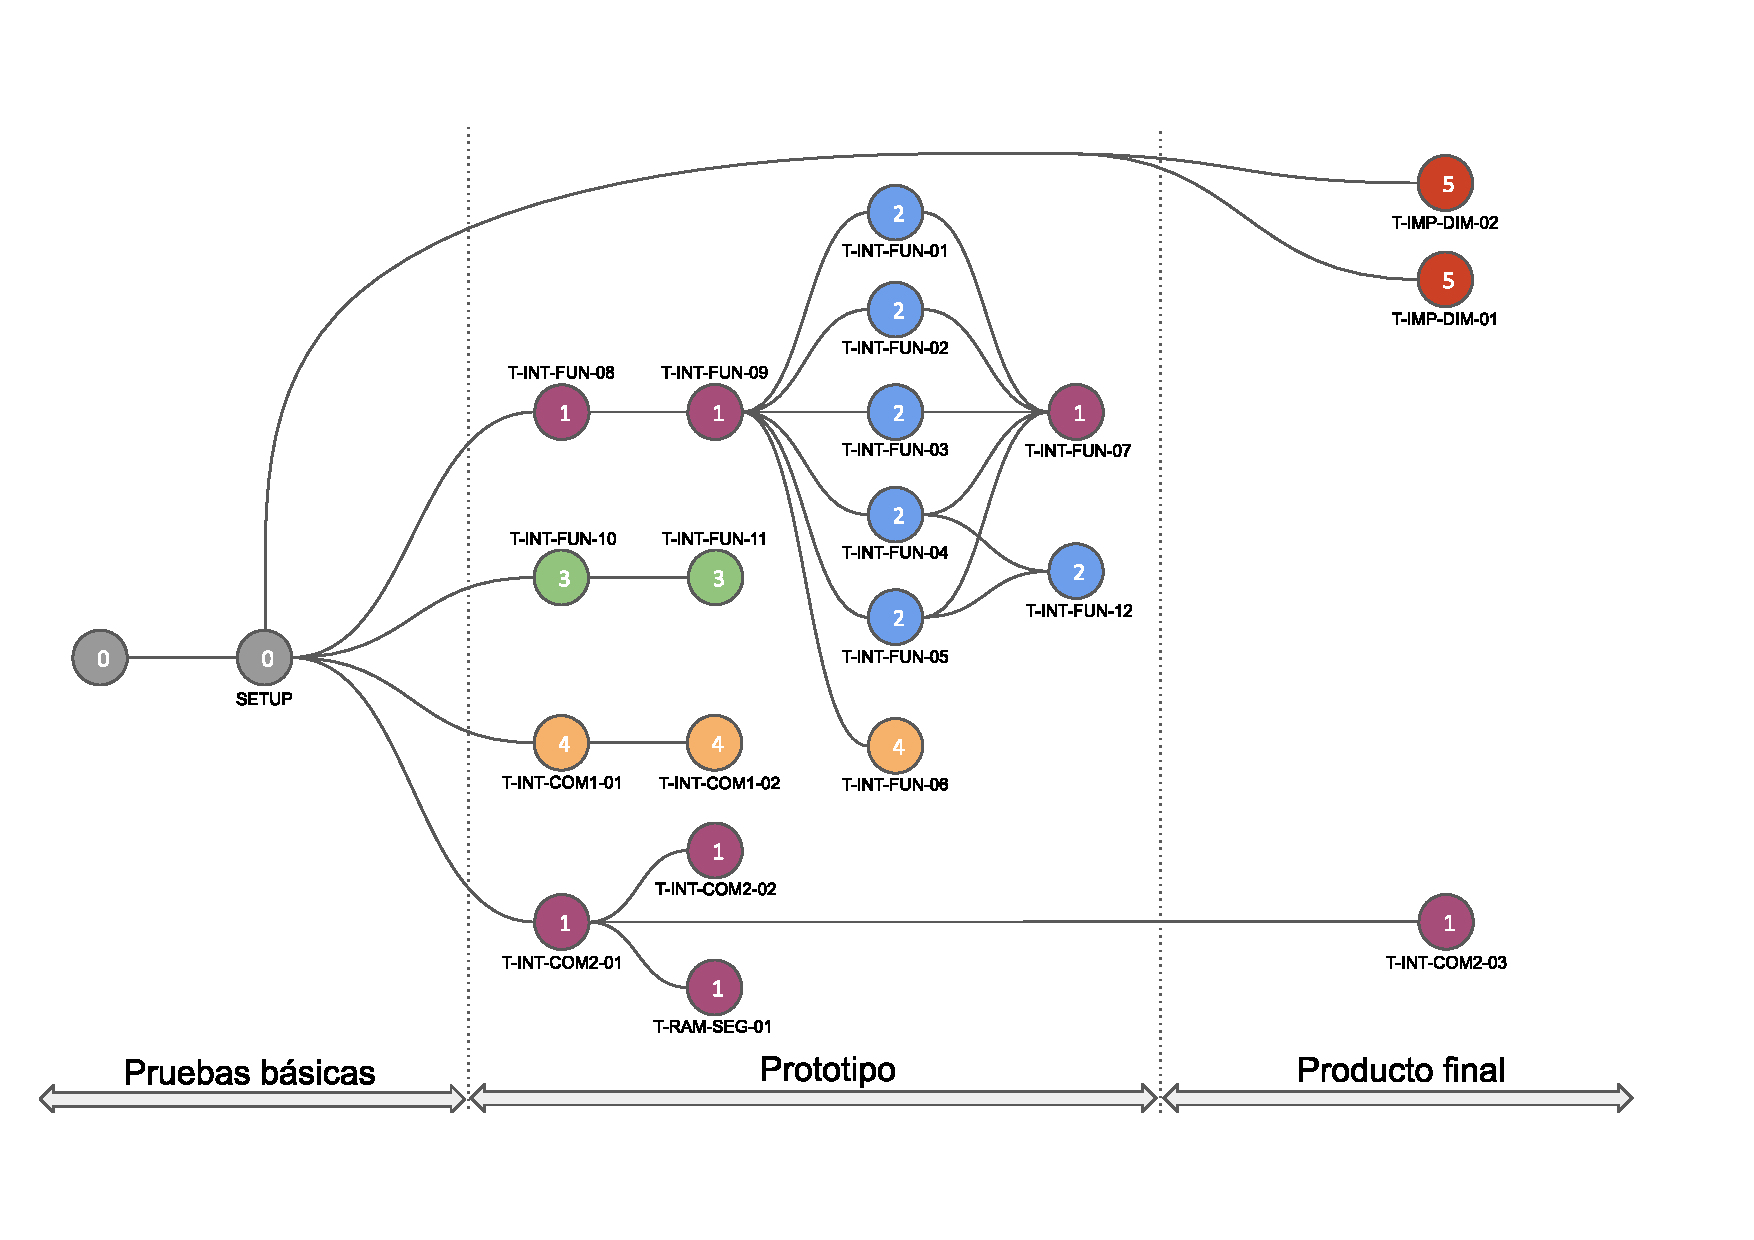
\includegraphics[width=0.9\linewidth,page=1]{ImagenesPlan de validacion/Diagrama de Dependencias de Validacion}
	\caption{Diagrama de dependencias del plan de validación.}
	\label{fig:diagrama_plan_validacion}
\end{figure}

%\end{document}